\documentclass[11pt]{article}
\usepackage{tikz}
\usepackage{geometry}
\usepackage{xcolor}

\geometry{verbose,tmargin=0.5in,bmargin=0.5in,lmargin=0.5in,rmargin=0.5in}

\usetikzlibrary{shapes,arrows,positioning,fit,backgrounds}

\begin{document}

\title{Telegram Bot CI/CD Workflow Diagram}
\maketitle

\begin{figure}[h]
\centering
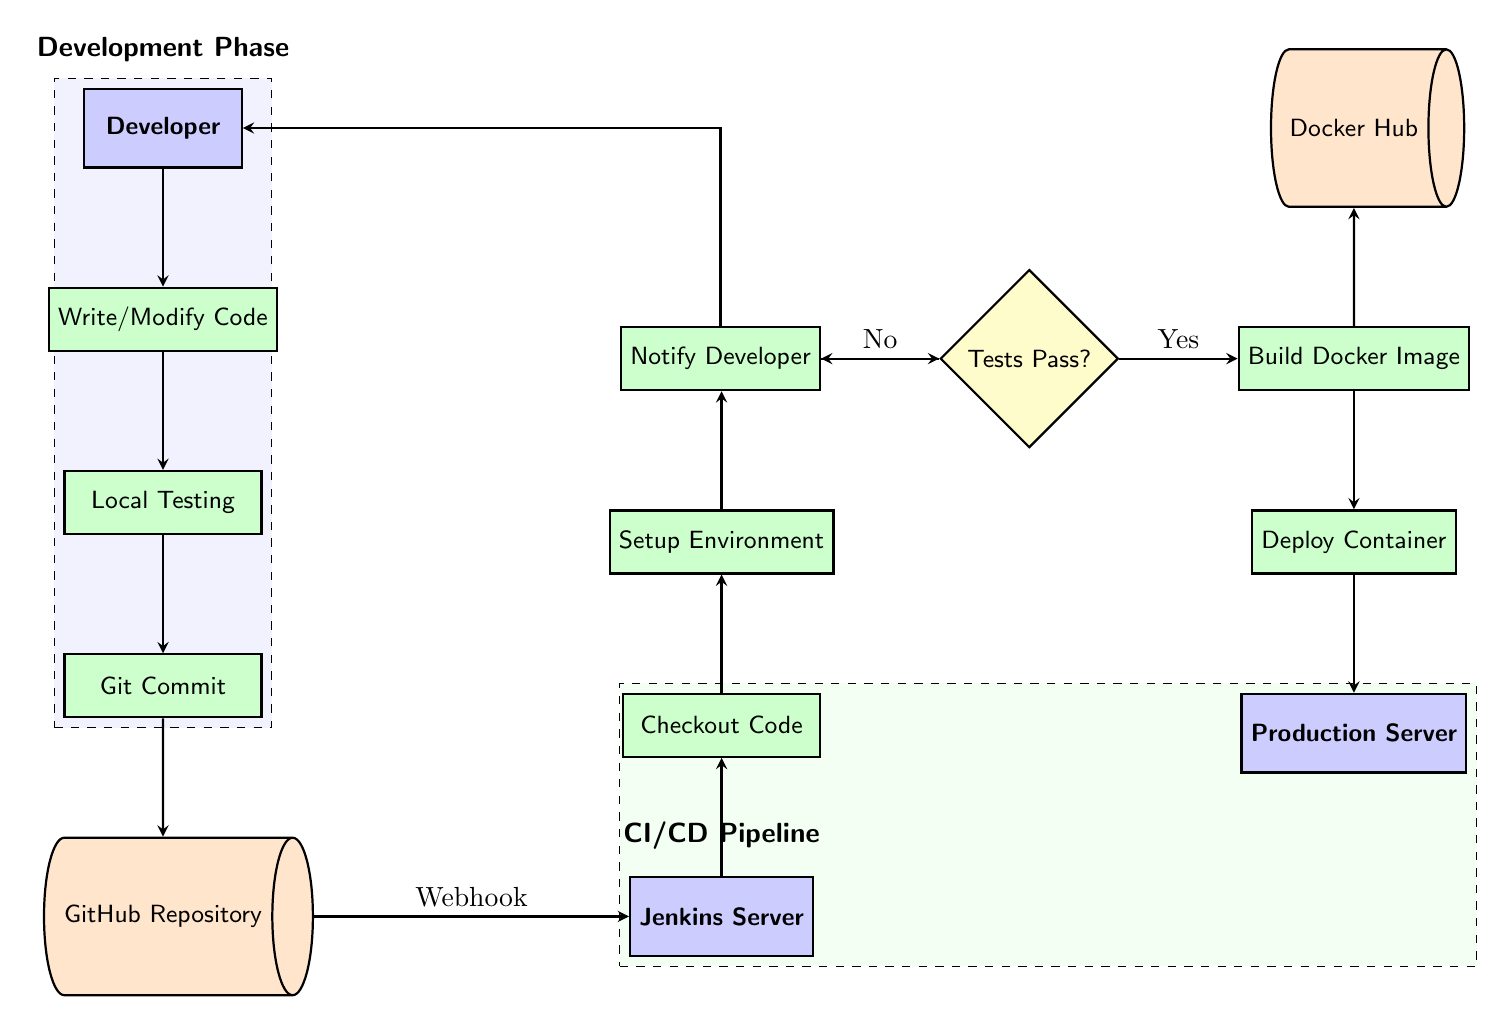
\begin{tikzpicture}[
    node distance=1.5cm,
    auto,
    thick,
    main node/.style={rectangle,fill=blue!20,draw,font=\sffamily\small\bfseries,minimum width=2cm,minimum height=1cm},
    process/.style={rectangle,fill=green!20,draw,font=\sffamily\small,minimum width=2.5cm,minimum height=0.8cm},
    decision/.style={diamond,fill=yellow!20,draw,font=\sffamily\small,minimum width=1.5cm,minimum height=1cm},
    storage/.style={cylinder,fill=orange!20,draw,font=\sffamily\small,minimum width=2cm,minimum height=1cm},
    arrow/.style={->,>=stealth,thick}
]

% Developer workflow
\node[main node] (dev) {Developer};
\node[process, below=of dev] (code) {Write/Modify Code};
\node[process, below=of code] (test) {Local Testing};
\node[process, below=of test] (commit) {Git Commit};
\node[storage, below=of commit] (github) {GitHub Repository};

% CI/CD Pipeline
\node[main node, right=4cm of github] (jenkins) {Jenkins Server};
\node[process, above=of jenkins] (checkout) {Checkout Code};
\node[process, above=of checkout] (setup) {Setup Environment};
\node[process, above=of setup] (validate) {Code Validation};
\node[decision, right=of validate] (testpass) {Tests Pass?};
\node[process, right=of testpass] (build) {Build Docker Image};
\node[storage, above=of build] (dockerhub) {Docker Hub};
\node[process, below=of build] (deploy) {Deploy Container};
\node[main node, below=of deploy] (production) {Production Server};

% Error handling
\node[process, left=of testpass] (notify) {Notify Developer};

% Arrows
\draw[arrow] (dev) -- (code);
\draw[arrow] (code) -- (test);
\draw[arrow] (test) -- (commit);
\draw[arrow] (commit) -- (github);
\draw[arrow] (github) -- node[midway,above] {Webhook} (jenkins);
\draw[arrow] (jenkins) -- (checkout);
\draw[arrow] (checkout) -- (setup);
\draw[arrow] (setup) -- (validate);
\draw[arrow] (validate) -- (testpass);
\draw[arrow] (testpass) -- node[midway,above] {Yes} (build);
\draw[arrow] (testpass) -- node[midway,above] {No} (notify);
\draw[arrow] (build) -- (dockerhub);
\draw[arrow] (build) -- (deploy);
\draw[arrow] (deploy) -- (production);
\draw[arrow] (notify) |- (dev);

% Background boxes
\begin{scope}[on background layer]
\node[fill=blue!5,draw,dashed,fit=(dev)(commit)] {};
\node[fill=green!5,draw,dashed,fit=(jenkins)(production)] {};
\end{scope}

% Labels
\node[above=0.2cm of dev, font=\sffamily\bfseries] {Development Phase};
\node[above=0.2cm of jenkins, font=\sffamily\bfseries] {CI/CD Pipeline};

\end{tikzpicture}
\caption{Complete CI/CD Workflow for Telegram Bot Project}
\end{figure}

\newpage

\section{Workflow Steps Description}

\subsection{Development Phase}
\begin{enumerate}
    \item \textbf{Developer} - Initiates the development process
    \item \textbf{Write/Modify Code} - Creates or updates Python bot functionality
    \item \textbf{Local Testing} - Tests bot locally with virtual environment
    \item \textbf{Git Commit} - Commits changes to local repository
    \item \textbf{GitHub Repository} - Pushes code to remote repository
\end{enumerate}

\subsection{CI/CD Pipeline Phase}
\begin{enumerate}
    \item \textbf{Jenkins Server} - Receives webhook notification from GitHub
    \item \textbf{Checkout Code} - Downloads latest code from repository
    \item \textbf{Setup Environment} - Creates Python virtual environment
    \item \textbf{Code Validation} - Runs syntax checks and tests
    \item \textbf{Tests Pass?} - Decision point for pipeline continuation
    \item \textbf{Build Docker Image} - Creates containerized application
    \item \textbf{Docker Hub} - Stores built images in registry
    \item \textbf{Deploy Container} - Deploys to production environment
    \item \textbf{Production Server} - Final deployment target
\end{enumerate}

\subsection{Error Handling}
\begin{itemize}
    \item \textbf{Notify Developer} - Sends failure notifications
    \item \textbf{Feedback Loop} - Returns to development phase for fixes
\end{itemize}

\end{document}